\documentclass[10pt]{report}
\usepackage{/Users/bradenhoagland/latex/math}

\lhead{Braden Hoagland}
\chead{HW 2}
\rhead{}

\renewcommand{\theenumi}{\alph{enumi}}

\begin{document}
%\tableofcontents

\begin{exer}[1.7: 4]
	Let $F(u,v) = (u^2-v^2, 2uv)$. Find a formula for the Jacobian matrix of $F$ at all points, and deduce that $F_{*\mathbf{p}}$ is a linear isomorphism at every point of $\mathbb{R}^2$ except the origin.
\end{exer}
The Jacobian matrix of $F$ at a point $\mathbf{p}=(p_1, p_2)$ is
\[
\begin{pmatrix}
	\frac{\partial f_1}{\partial u}(\mathbf{p}) & \frac{\partial f_1}{\partial v} (\mathbf{p})\\[6pt]
	\frac{\partial f_2}{\partial u} (\mathbf{p})& \frac{\partial f_2}{\partial v} (\mathbf{p})
\end{pmatrix} =
\begin{pmatrix}
	2p_1 & -2p_2 \\
	2p_2 & 2p_1
\end{pmatrix}.
\] We already know that $F_{*\mathbf{p}}$ is linear, so it is a vector space homomorphism. If $\mathbf{p}=\mathbf{0}$, then the Jacobian has rank 0; however, if $\mathbf{p} \neq \mathbf{0}$, then the Jacobian reduces to $I_2$ by Gaussian elimination, meaning that it has full rank. Thus when $\mathbf{p}$ is nonzero, $F_{*\mathbf{p}}$ is one-to-one. Since $F_{*\mathbf{p}}$ is a linear map between vector spaces that are both dimension 2 ($T_{\mathbf{p}}(\mathbb{R}^2)$ and $T_{F(\mathbf{p})}(\mathbb{R}^2)$ are both isomorphic to $\mathbb{R}^2$), it is automatically also onto. Thus $F_{*\mathbf{p}}$ is linear isomorphism at all points other than the origin.

\begin{exer}[2.1: 3]
Prove that the tangent vectors
\[
	\mathbf{e}_1 = \frac{(1,2,1)}{\sqrt{6} }, \mathbf{e}_2=\frac{(-2,0,2)}{\sqrt{8} }, \mathbf{e}_3=\frac{(1,-1,1)}{\sqrt{3} } 
\] constitute a frame. Express $\mathbf{v}=(6,1,-1)$ as a linear combination of these vectors.
\end{exer}
Since $\Vert{\mathbf{e}_1}\Vert = \sqrt{1+4+1} /\sqrt{6} =1$, $\Vert{\mathbf{e}_2}\Vert=\sqrt{4+0+4} /\sqrt{8} =1$, and $\Vert{\mathbf{e}_3}\Vert=\sqrt{1+1+1} /\sqrt{3} =1$, all three vectors are unit vectors. Additionally, their dot products are
\begin{align*}
	\mathbf{e}_1\cdot \mathbf{e}_2 &= \frac{-2+0+2}{\sqrt{6} \sqrt{8} } =0 \\
	\mathbf{e}_1 \cdot \mathbf{e}_3 &= \frac{1-2+1}{\sqrt{6} \sqrt{3} } =0 \\
	\mathbf{e}_2 \cdot \mathbf{e}_3 &= \frac{-2+0+2}{\sqrt{8} \sqrt{3} } =0,
\end{align*}
so they are mutually orthogonal. Thus $\mathbf{e}_1, \mathbf{e}_2, \mathbf{e}_3$ forms a frame.

We can express $\mathbf{v}$ as a linear combination of this frame by
\begin{align*}
	\mathbf{v} &= \frac{7 \sqrt{6} }{6} \mathbf{e}_1 - \frac{7\sqrt{8} }{4} \mathbf{e}_2 + \frac{4\sqrt{3} }{3} \mathbf{e}_3 \\
		   &= \left( \frac{7}{6} , \frac{14}{6} , \frac{7}{6}  \right)-\left( -\frac{14}{4} , 0, \frac{14}{4}  \right) + \left( \frac{4}{3} , -\frac{4}{3} , \frac{4}{3}  \right) \\
		   &= (6, 1, -1).
\end{align*}

\begin{exer}[2.1: 9]
	Prove, using $\varepsilon$-neighborhoods, that each of the following subsets of $\mathbb{R}^3$ is open:
	\begin{enumerate}
		\item All points $\mathbf{p}$ such that $\Vert{\mathbf{p}}\Vert<1$.
		\item All $\mathbf{p}$ such that $p_3>0$.
	\end{enumerate}
\end{exer}
\begin{enumerate}
	\item Let $A$ denote the set of all points with norm less than 1, and let $\mathbf{p} \in A$. Then $\Vert{\mathbf{p}}\Vert=d$ for some $d < 1$. We claim that the ball $B(\mathbf{p}, 1-d)$ is contained in $A$. Let $\mathbf{q} \in B(\mathbf{p}, 1-d)$, then
		\[
		\Vert{\mathbf{q}}\Vert= \Vert{\mathbf{q}-\mathbf{p}+\mathbf{p}}\Vert\leq \Vert{\mathbf{q}-\mathbf{p}}\Vert+\Vert{\mathbf{p}}\Vert < 1-d+d = 1.
	\] Thus $B(\mathbf{p}, 1-d) \subset A$. Since $\mathbf{p}$ was arbitrary, this shows that $A$ is open.

\item Let $B$ denote the set of all points whose 3rd coordinate is positive. Let $\mathbf{p} \in B$, then $p_3=d>0$. We claim that the ball $B(\mathbf{p},d)$ is contained in $B$. Let $\mathbf{q} \in B(\mathbf{p},d)$, then
	\[
	|q_3-p_3| \leq \Vert{\mathbf{q}-\mathbf{p}}\Vert<d,
\] so $q_3 > 0$. Since $\mathbf{p}$ was arbitrary, this shows that $B$ is open.
\end{enumerate}

\begin{exer}[2.3: 1]
	Compute the \textbf{Frenet apparatus} $\kappa, \tau, T, N, B$ of the unit-speed curve
	\[
		\beta(s) = \left( \frac{4}{5} \cos s, 1-\sin s, -\frac{3}{5} \cos s \right).
	\] Show that this curve is a circle; find its center and radius.
\end{exer}
The tangent vector field is
\[
	T(s) = \beta'(s) = \left( -\frac{4}{5} \sin s, -\cos s, \frac{3}{5} \sin s \right).
\] The curvative is then
\[
	\kappa(s) = \Vert{T'(s)}\Vert = \frac{16}{25} \cos^2 s + \sin^2 s + \frac{9}{25} \cos^2 s = 1.
\] The principal normal vector field is
\[
	N(s) = T'(s) / \kappa(s) = T'(s) = \left( -\frac{4}{5} \cos s, \sin s, \frac{3}{5} \cos s \right).
\] The binormal vector field is
\begin{align*}
	B = T \times N &= \left| 
	\begin{matrix}
		U_1 & U_2 & U_3 \\
		-4/5\;\sin & -\cos & 3/5\;\sin \\
		-4/5\cos & \sin & 3/5\;\cos
	\end{matrix}\right| \\
		       &= \left( -\frac{3}{5} \cos^2 - \frac{3}{5} \sin^2 \right)U_1 + \left( -\frac{4}{5} \sin^2 - \frac{4}{5} \cos^2 \right)U_3 \\
		       &= \left( -\frac{3}{5}, 0, -\frac{4}{5} \right).
\end{align*}
Then since $B' = -\tau N$, $B' = 0$, and $N$ is not everywhere 0, the torsion $\tau$ must be 0.

Since $\kappa$ is a positive constant and $\tau=0$, $\beta$ is part of a circle of radius $1/\kappa = 1$. Its center is
\[
	\beta(s) + \frac{1}{\kappa(s)} N(s) = \beta(s) + N(s) = (0, 1, 0).
\] 

\begin{exer}[2.3: 5]
	If $A$ is a vector field $\tau T+\kappa B$ on a unit-speed curve $\beta$, show that the Frenet formulas become
	\begin{align*}
		T' &= A \times T, \\
		N' &= A \times N, \\
		B' &= A \times B.
	\end{align*}
\end{exer}
Since $N=B\times T$,
\[
	A \times T = (T \times T) + \kappa(B \times T) = 0 + \kappa N = T'.
\] 
Since $B=T \times N$, $T = N \times B$, and the cross product is antisymmetric,
\[
	A \times N = \tau(T \times N) + \kappa(B\times N) = \tau B - \kappa T = N'.
\] 
Finally, since $N = B \times T = - T \times B$,
\[
	A \times B = \tau (T \times B) + \kappa(B \times B) = -\tau N = B'.
\] 

\begin{exer}[2.3: 6]
A unit-speed parameterization of a circle may be written
\[
	\gamma(s) = \mathbf{c} + r\cos \frac{s}{r} \mathbf{e}_1 + r \sin \frac{s}{r} \mathbf{e}_2,
\] where $\mathbf{e}_i \cdot \mathbf{e}_j = \delta_{ij}$.

If $\beta$ is a unit-speed curve with $\kappa(0)>0$, prove that there is one and only one circle $\gamma$ that approximates $\beta$ near $\beta(0)$ in the sense that
\[
	\gamma(0)=\beta(0), \quad \gamma'(0) = \beta'(0), \quad \text{and } \gamma''(0) = \beta''(0).
\] Show that $\gamma$ lies in the osculating plane of $\beta$ at $\beta(0)$ and find its center $\mathbf{c}$ and radius $r$.
\end{exer}
Assuming that $\gamma$ matches $\beta$ and its first two derivatives at $s=0$, we can take the derivative of $\gamma$ and evaluate at $s=0$ to get
\begin{align*}
	\gamma'(s) &= -\sin\left( \frac{s}{r}  \right)\mathbf{e}_1 + \cos\left( \frac{s}{r}  \right)\mathbf{e}_2 \\
	\gamma'(0) &= -\sin(0) \mathbf{e}_1 + \cos(0)\mathbf{e}_2 \\
	T(0) = \beta'(0) &= \mathbf{e}_2,
\end{align*}
which gives us the first component of the osculating circle's frame. Differentiating again gives
\begin{align*}
	\gamma''(s) &= -\frac{1}{r} \cos\left(  \frac{s}{r} \right)\mathbf{e}_1 - \frac{1}{r} \sin\left( \frac{s}{r}  \right)\mathbf{e}_2 \\
	\gamma''(0) &= -\frac{1}{r} \cos(0) \mathbf{e}_1 - \frac{1}{r} \sin(0) \mathbf{e}_2 \\
	\kappa(0)N(0) = T'(0) = \beta''(0) &= -\frac{1}{r} \mathbf{e}_1.
\end{align*}
Since $\kappa(s)$ is strictly greater than 0 for all $s$, this implies that $\mathbf{e}_1=-N(0)$ and $r=1/\kappa(0)$. Plugging these into the original form of the circle at $s=0$ gives
\begin{align*}
	\beta(0) = \gamma(0) &= \mathbf{c} - \frac{1}{\kappa(0)} \cos(0)N(0) + \frac{1}{\kappa(0)} \sin(0) T \\
			     &= \mathbf{c} - \frac{1}{\kappa(0)} N(0).
\end{align*}
Simply rearranging this shows that the center of the circle is $\mathbf{c}=\beta(0) + \frac{1}{\kappa(0)} N(0)$. We have found a circle that matches $\beta$ and its first two derivatives at $s=0$, and since it is defined totally in terms of the unique values $T(0), N(0),$ and $\kappa(0)$, we know the circle itself is unique. Finally, we note that since our circle is defined in terms of $N(0)$ and $T(0)$, it lies in the osculating plane of $\beta$ at $\beta(0)$.

\begin{exer}[2.3: 7]
	If $\alpha$ and a reparameterization $\overline{\alpha} =\alpha(h)$ are both unit-speed curves, show that
	\begin{enumerate}
		\item $h(s)=\pm s + s_0$ for some number $s_0$;
		\item $\overline{T} = \pm T(h)$, $\overline{N}=N(h), \overline{\kappa} =\kappa(h)$, $\overline{\tau} =\tau(h)$, and $\overline{B}=\pm B(h)$,
	\end{enumerate}
	where the sign $(\pm)$ is the same as that in (a), and we assume $\kappa>0$.
\end{exer}
\begin{enumerate}
	\item The speed of the reparameterization is $\Vert{\overline{\alpha}'}\Vert= \Vert{\alpha'(h)}\Vert \Vert{h'}\Vert = 1$, but we are also given that $\Vert\alpha\Vert=1$, so it must be the case that $h'=\pm 1$. The only functions $h$ that satisfy this everywhere are of the form $h(s) = \pm s + s_0$, since the added constant term does not affect the derivative.

	\item These derivations are straightforward applications of the fact that $h' = \pm 1$. The unit tangent vector field is
		\[
			\overline{T}=\overline{\alpha}' = \alpha'(h)h' = T(h)h' = \pm T(h).
		\] Then the curvature is
		\[
			\overline{\kappa} = \Vert{\overline{T}'}\Vert=\Vert{\pm T'(h)h'}\Vert=\Vert{T'(h)}\Vert=\kappa(h),
		\] so the principal normal vector field is
		\[
			\overline{N}=\frac{\overline{T}'}{\overline{\kappa}} = \frac{\pm T'(h)h'}{\kappa(h)} = \frac{T'(h)}{\kappa(h)} = N(h).
		\] The binormal vector field is
		\[
			\overline{B}= \overline{T}\times \overline{N} = \pm T(h) \times N(h) = \pm B(h),
		\] which means the torsion is
		\[
			\overline{\tau} = -\frac{\overline{B}'}{\overline{N}} =-\frac{\pm B'(h) h'}{N(h)} = -\frac{B'(h)}{N(h)} = \tau(h).
		\] 
\end{enumerate}

\begin{exer}[2.3: 10]
Let $\alpha$ be a unit-speed curve with $\kappa>0$, $\tau \neq 0$.
\begin{enumerate}
	\item If $\alpha$ lies on a sphere of center $\mathbf{c}$ and radius $r$, show that
		\[
		\alpha-\mathbf{c} = -\rho N - \rho' \sigma B,
	\] where $\rho=1/\kappa$ and $\sigma=1/\tau$. Thus $r^2 = \rho^2+(\rho'\sigma)^2$.
\item Conversely, if $\rho^2+(\rho'\sigma)^2$ has constant value $r^2$ and $\rho'\neq 0$, show that $\alpha$ lies on a sphere of radius $r$.
\end{enumerate}
\end{exer}
\begin{enumerate}
	\item We can express any vector $\mathbf{v}$ in terms of the Frenet frame by
		\[
			\mathbf{v} = (\mathbf{v}\cdot T)T + (\mathbf{v}\cdot N)N + (\mathbf{v}\cdot B)B,
		\] so need to calculate each of these dot products for $\mathbf{v} = \alpha-\mathbf{c}$. Since $\alpha$ lies on a sphere with center $\mathbf{c}$ and radius $r$, we know
		\[
			r^2 = \Vert{\alpha-\mathbf{c}}\Vert^2 = (\alpha-\mathbf{c})\cdot(\alpha-\mathbf{c}).
		\] We can differentiate this several times and use the Frenet formulas to derive our desired dot product expressions. Taking the first derivative yields
		\begin{align*}
			0 &= 2(\alpha-\mathbf{c})'\cdot (\alpha-\mathbf{c}) \\
			  &= 2T \cdot (\alpha-c),
		\end{align*}
		from which we get $T \cdot (\alpha-\mathbf{c})=0$. Differentiating this and using the Frenet formula for $T'$ gives
		\begin{align*}
			0 &= T' \cdot (\alpha-\mathbf{c}) + T\cdot T \\
			  &= \kappa N \cdot (\alpha-\mathbf{c}) + 1,
		\end{align*}
		from which we get $N \cdot (\alpha-\mathbf{c}) = -1/\kappa = -\rho$. Differentiating this and using the Frenet formula for $N'$ gives
		\begin{align*}
			0 &= \kappa' N \cdot (\alpha-\mathbf{c}) + kN'\cdot (\alpha-\mathbf{c}) + \kappa N\cdot T \\
			  &= -\kappa' \frac{1}{\kappa} + \kappa(\tau B-\kappa T) \cdot (\alpha-\mathbf{c}) + 0.
			  \intertext{using the just-derived fact that $T$ and $(\alpha-\mathbf{c})$ are orthogonal, this simplifies to}
			  0 &= -\frac{\kappa'}{\kappa} + \kappa\tau B\cdot(\alpha-\mathbf{c}) \\
			  \intertext{which can be rearranged into}
			  B \cdot (\alpha-\mathbf{c}) &= \frac{\kappa'}{\kappa^2} \frac{1}{\tau} = -\left( \frac{1}{\kappa}  \right)' \frac{1}{\tau} = -\rho' \sigma.
		\end{align*}
		Now that we've calculated each of the dot products that we needed, we can write $\alpha-\mathbf{c}$ in terms of the Frenet frame as
		\[
		\alpha-\mathbf{c} = -\rho N - \rho' \sigma B.
		\] 

	\item We are given that $\rho^2 + (\rho'\sigma)^2 = r^2$, so we can differentiate this to gain more information:
		\begin{align*}
			2\rho \rho' + 2\rho' \sigma[\rho'\sigma' + \rho''\sigma] & 0 \\
			\rho'\sigma' + \rho''\sigma &= -\frac{\rho}{\sigma} .
		\end{align*}
		We can use this identity to show that the curve $\gamma = \alpha + \rho N + \rho' \sigma B$ is constant. Differentiating $\gamma$ and substituting in the Frenet formulas yields
		\begin{align*}
			\gamma' &= T + \rho' N + \rho N' + \rho'' \sigma B + \rho' \sigma' B + \rho' \sigma B' \\
				&= [1 - \rho \kappa] T + [\rho' - \rho' \sigma \tau] N + [\rho\tau + \rho'' \sigma + \rho'\sigma'] B \\
				&= [1-1] T + [\rho' - \rho'] N + [\rho / \sigma - \rho / \sigma] B \\
				&= 0.
		\end{align*}
		Thus $\gamma$ is a constant curve, i.e. a point, which we can choose to call $\mathbf{c}$. Then
		\begin{align*}
			\Vert{\alpha-\mathbf{c}}\Vert^2 = \Vert{-\rho N + \rho'\sigma B}\Vert^2 = \rho^2 + (\rho'\sigma)^2 = r^2,
		\end{align*}
		so $\alpha$ lies on the sphere centered at $\mathbf{c}$ of radius $r$.

\end{enumerate}

\begin{exer}[2.4: 4]
Show that the curvature of a regular curve in $\mathbb{R}^3$ is given by
\[
	\kappa^2 v^4 = \Vert{\alpha''}\Vert^2 - \left(\frac{d v}{d t}\right)^2.
\] 
\end{exer}
Since $\alpha'' = \frac{d v}{d t} T + \kappa v^2 N$, we have
\begin{align*}
	\Vert{\alpha''}\Vert^2 - \left( \frac{d v}{d t}  \right)^2 &= \left\Vert{\frac{d v}{d t} T + \kappa v^2 N}\right\Vert - \left( \frac{d v}{d t}  \right)^2 \\
								   &= \left( \frac{d v}{d t}  \right)^2+\kappa^2 v^4 - \left( \frac{d v}{d t}  \right)^2 \\
								   &= \kappa_{62} v^4.
\end{align*}

\begin{exer}[2.4: 16]
Let
\[
	f(t) =
	\begin{cases}
		0 & t \leq 0,\\
		e^{-1/t^2} & t > 0
	\end{cases}
\] and let
\[
	\alpha(t) = (t, f(t), f(-t)).
\]
\begin{enumerate}
	\item Sketch $\alpha$ on an interval $-a \leq t \leq a$.
	\item Show that the curvature of $\alpha$ is zero only at $t=0$.
	\item What are the osculating planes of $\alpha$ for $t < 0 $ and $t>0$?
\end{enumerate}
\end{exer}
\begin{enumerate}
	\item Below is a sketch of $\alpha$ over the interval $-a \leq t \leq a$. As I've tried to indicate with shading, the portion of the curve with $t>0$ lies entirely in the $x-y$ plane, and the portion of the curve with $t<0$ lies entirely in the $x-z$ plane.
		\begin{figure}[H]
			\centering
			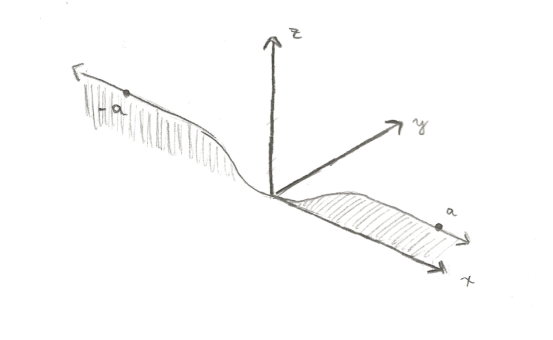
\includegraphics[scale=0.9]{fig/curve.pdf}
		\end{figure}
		

	\item The curvature can be calculated as $\kappa=\Vert{\alpha' \times \alpha''}\Vert/\Vert{\alpha'}\Vert^3$. Since
		\[
			\Vert{\alpha'(t)}\Vert = \sqrt{1 + (f'(t))^2 + (f'(-t))^2} \geq \sqrt{1} =1,
		\] there can never be division by 0. Thus this question reduces to showing that $\Vert{\alpha' \times \alpha''}\Vert=0$ only when $t=0$.

		We have
		\begin{align*}
			\alpha'(t) \times \alpha''(t) &= \left| 
			\begin{matrix}
				U_1 & U_2 & U_3 \\
				1 & f'(t) & -f'(-t) \\
				0 & f''(t) & f''(-t)
			\end{matrix}\right| \\
						      &= \left( f'(t)f''(-t) + f'(-t)f''(t) \right)U_1 - f''(-t)U_2 + f''(t)U_3,
		\end{align*}
		which has norm
		\[
			\Vert{\alpha'(t)\times \alpha''(t)}\Vert = \sqrt{[f'(t)f''(-t) + f'(-t)f''(t)]^2 + f''(-t)^2 + f''(t)^2} .
		\] 

		We calculate that when $t>0$,
		\begin{align*}
			f'(t) &= 2t^{-3}e^{-1/t^2} \\
			f''(t) &= e^{-1/t^2}(4t^{-6}-et^{-4}).
		\end{align*}
		When $t\leq 0$, both $f'$ and $f''$ evaluate to 0. The important part of these calculations is not the formulas themselves, but rather the fact that if $t$ is strictly positive, then $f'(t)$ and $f''(t)$ are both nonzero.

		Now for $t=0$, every term in norm becomes 0, so the norm overall is 0. If $t > 0$, then $f''(-t)=f'(-t)=0$, so the norm reduces to $|f''(t)|$. Similarly, when $t<0$, the norm reduces to $|f''(-t)|$. In these latter two cases, $t$ and $-t$ are both strictly positive, so $f''$ is nonzero. Thus the curvature is zero only when $t=0$.

	\item The osculating plane is spanned by vectors parallel to $T$ and $N$, so we find such vectors by calculating $\alpha'$ (parallel to $T$) and $\alpha''$ (parallel to $N$). We can also describe the planes with a single vector that is orthogonal to the plane.

		When $t>0$, we have
		\begin{align*}
			\alpha' &= (1, f', 0) \\
			\alpha'' &= (0, f'', 0),
		\end{align*}
		so these two vectors span the osculating plane at $\alpha(t)$. Since neither vector has a nonzero third component, the osculating plane is clearly perpendicular to $(0, 0, 1)$, i.e. it is the $x-y$ plane.

		When $t<0$, we have
		\begin{align*}
			\alpha' &= (1, 0, -f') \\
			\alpha'' &= (0, 0, -f'').
		\end{align*}
		With similar reasoning as before, the osculating plane is perpendicular to $(0, 1, 0)$, i.e. it is the $x-z$ plane.
\end{enumerate}


\end{document}
